  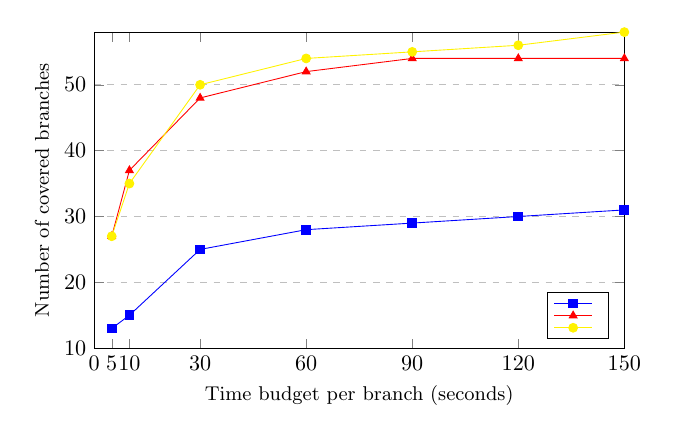
\begin{tikzpicture}[scale=0.8]
    \begin{axis}[
        xlabel={Time budget per branch (seconds)},
        ylabel={Number of covered branches},
        width=10cm,height=6.6cm,
        xmin=0, xmax=150,
        ymin=10, ymax=58,
        xtick={0,5,10,30,60,90,120,150,180},
        ytick={0,10,20,30,40,50},
        legend pos=south east,
        ymajorgrids=true,
        % xmajorgrids=true,
        grid style=dashed,
        label style={font=\small}
      ]

      \addplot[
        color=blue,
        mark=square*,
      ] coordinates {
        (5,13) (10,15) (30,25) (60,28) (90,29) (120,30) (150,31)
      };
      \addplot[
        color=red,
        mark=triangle*,
      ]  coordinates {
        (5,27) (10,37) (30,48) (60,52) (90,54) (120,54) (150,54)
      };
      \addplot[
        color=yellow,
        mark=*,
      ]   coordinates {
        (5,27) (10,35) (30,50) (60,54) (90,55) (120,56) (150,58)
      };
      \legend{$\Random$,$\Genetic$,$\RGenetic$}

    \end{axis}
  \end{tikzpicture}
